\documentclass[11pt, letterpaper]{article}
\input{/home/hyperion/.config/LatexHub/preambles/base.tex}
\input{/home/hyperion/.config/LatexHub/preambles/diagrams.tex}
\input{/home/hyperion/.config/LatexHub/preambles/tikz.tex}
\input{/home/hyperion/.config/LatexHub/preambles/code.tex}
\input{/home/hyperion/.config/LatexHub/preambles/macros-cat-theory.tex}
\input{/home/hyperion/.config/LatexHub/preambles/macros-algebra.tex}
\input{/home/hyperion/.config/LatexHub/preambles/basic-theorems-section.tex}
\input{/home/hyperion/.config/LatexHub/preambles/refs-basic.tex}
\input{/home/hyperion/.config/LatexHub/preambles/homework-formatting.tex}
\usepackage{titlepageBU}
\title{Problem Set 6}
\begin{document}
\makeproblem
\section{Problem 1}

As noted in equation 15.1.10, the potential is
\[
	V(r)=\frac{1}{2} -\frac{GM}{r} +\frac{\ell ^2}{2r^2} -\frac{GM\ell ^2}{r^3} 
.\]
Following the notes, we choose units such that $GM=1$, yielding potential
\[
	V(r)=\frac{1}{2} -\frac{1}{r} +\frac{\ell ^2}{2r^2} -\frac{\ell ^2}{r^3} 
.\]
Then
\[
	V'(r)=\frac{1}{r^2} -\frac{\ell ^2}{r^3} +\frac{3\ell ^2}{r^4} 
.\]
We can now directly solve the differential equations.
\begin{lstlisting}[language=Mathematica]
(* basic parameters *)
ell = 10;
rPlus = 1/2 (ell^2 + ell Sqrt[ell^2 - 12]);
r0 = 8 rPlus;

(* -V'(r) *)
rhs[r_] := -1/r^2 + ell^2/r^3 - (3 ell^2)/r^4;

(* have to wait till r'=0 the seconld time; the fisrt time is its closest approach *)
turnCount = 0;

(*solve the differential equation for like a few orbits *)
sol = NDSolve[{
    r''[lambda] == rhs[r[lambda]],
    phi'[lambda] == ell/r[lambda]^2,
    r[0] == r0,
    r'[0] == 0,
    phi[0] == 0
   },
   {r, phi},
   {lambda, 0, 300000},
   Events -> {
     WhenEvent[r'[lambda] == 0 && lambda > 10,
       {turnCount++, If[turnCount == 2, lambdaEnd = lambda]}
       ]
   }
];

rFun = r /. sol[[1]];
phiFun = phi /. sol[[1]];

phiFinal = phiFun[lambdaEnd];
precession = phiFinal - 2 Pi;
Print["Precession Angle: ", precession];
\end{lstlisting}
We obtain a precession angle of $0.206374$.
\begin{lstlisting}[language=Mathematica]

(* r(lambda) *)
Plot[rFun[l], {l, 0, 5.5 * lambdaEnd},
 AxesLabel -> {"\[Lambda]", "r"},
 PlotStyle -> Blue,
 GridLines -> Automatic]

(* phi(lambda) *)
Plot[phiFun[l], {l, 0, 5.5 * lambdaEnd},
 AxesLabel -> {"\[Lambda]", "\[Phi]"},
 PlotStyle -> Darker[Green],
 GridLines -> Automatic]

(* parametric orbit *)
ParametricPlot[{rFun[l] Cos[phiFun[l]], rFun[l] Sin[phiFun[l]]},
 {l, 0, 5.5 * lambdaEnd},
 AxesLabel -> {"x", "y"},
 PlotStyle -> Black, 
 PlotRange -> All,
 AspectRatio -> 1,
 GridLines -> Automatic]	
\end{lstlisting}
The figures are on another page because LaTeX formatting sucks.
\begin{figure}[ht]
	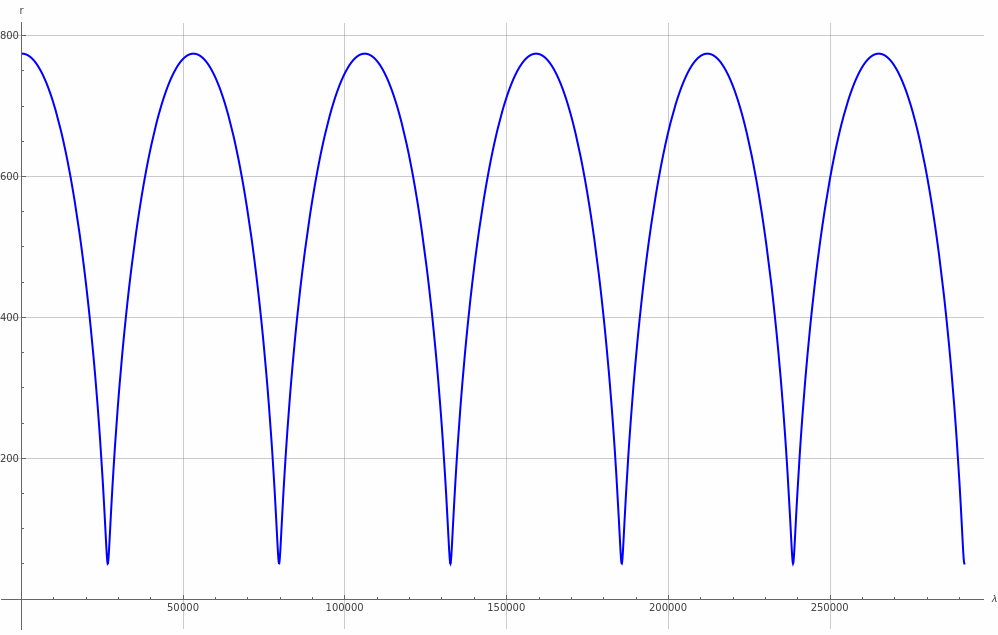
\includegraphics[scale=0.25]{../figures/lambda.png}
	\centering
	\caption{$r(\lambda )$ plotted against $\lambda $.}
	\centering
	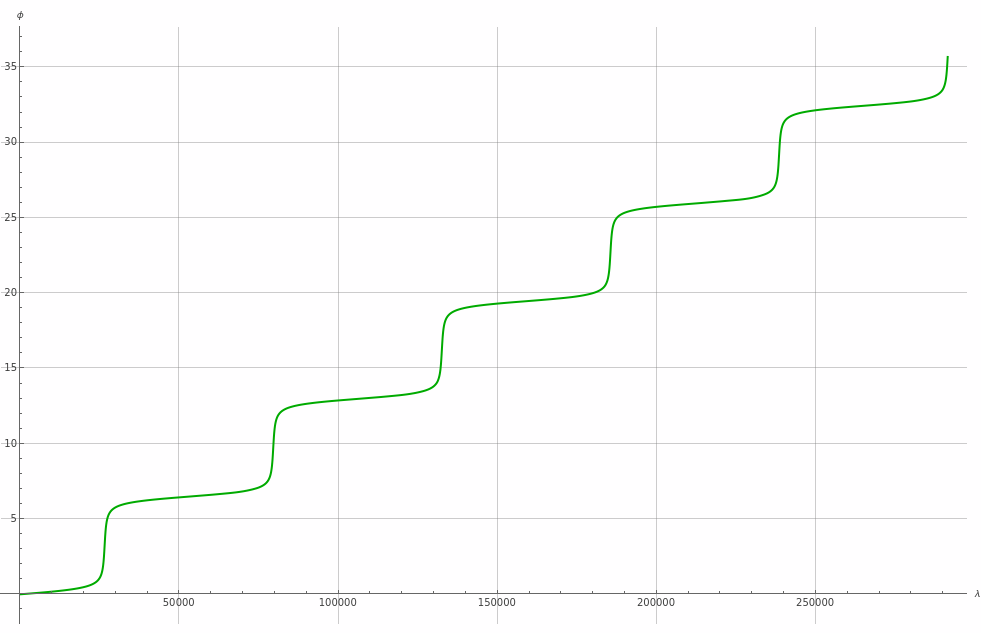
\includegraphics[scale=0.25]{../figures/phi.png}
	\centering
	\caption{$\phi(\lambda )$ plotted against $\lambda $.}
	\centering
	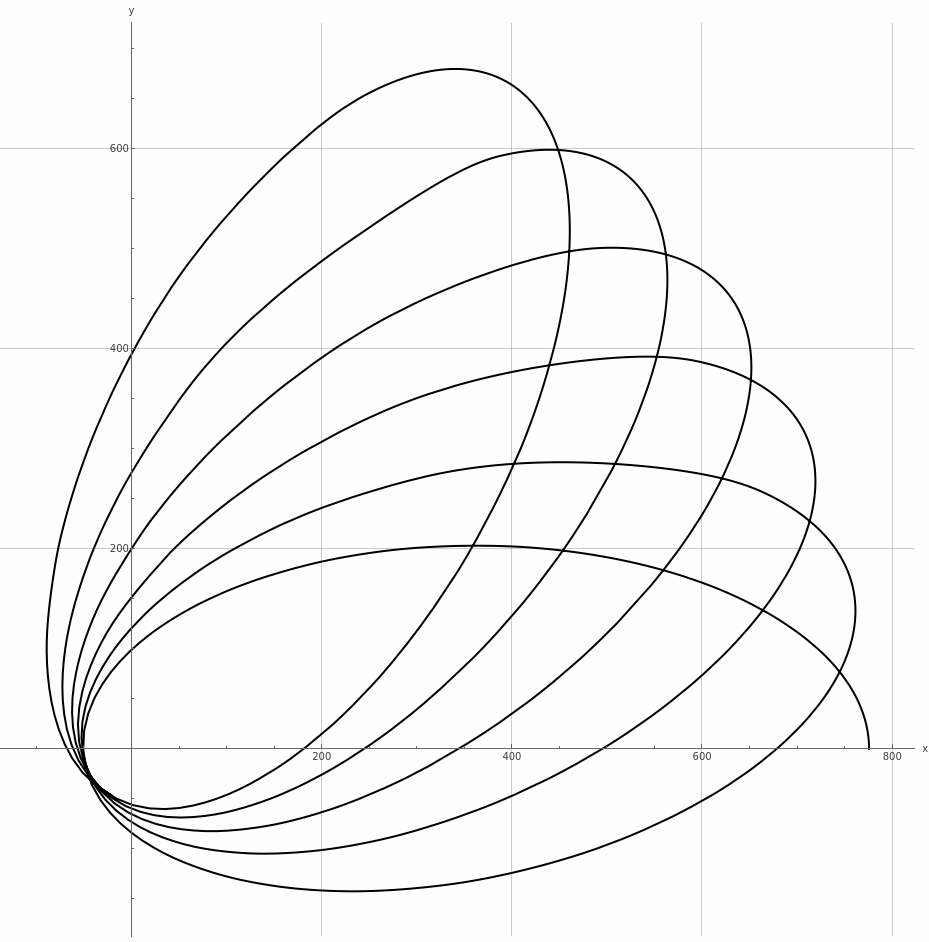
\includegraphics[scale=0.25]{../figures/parametric.png}
	\centering
	\caption{Parametric plot of the orbit.}
	\centering
\end{figure}

\end{document}
